\documentclass[12pt]{article}

\usepackage[margin=1in]{geometry}
\usepackage{amsmath}
\usepackage{amssymb}
\usepackage{graphicx}
\usepackage{apacite}
\usepackage{setspace}

\renewcommand{\baselinestretch}{2}

\newcommand{\clr}{\operatorname{clr}}
\newcommand{\N}{\operatorname{N}}
\newcommand{\cov}{\operatorname{cov}}
\newcommand{\var}{\operatorname{var}}

\DeclareMathOperator*{\argmin}{arg\,min}
\DeclareMathOperator{\tr}{tr}

\title{Limitations of Graph Selection from High-Dimensional Compositional Data}
\author{Camden Lopez \\ Master's Project Report \\ Department of Statistics, Oregon State University}
\date{May 30, 2017 \\ Corrected June 5, 2017}

\begin{document}
\pagenumbering{gobble}
\maketitle

\clearpage
\setcounter{page}{1}
\pagenumbering{arabic}

\subsection*{Introduction}

This work was motivated by the problem of inferring microbial interaction networks from compositional data. High-throughput sequencing methods such as 16S amplicon sequencing produce count data representing the abundances of microbial operational taxonomic units (OTUs) in a collection of samples. The counts are assumed to be proportional to the absolute abundances of the OTUs, but the sample preparation and sequencing process introduce biases such that the total sample counts do not accurately reflect the total abundance of microbes in the samples. Therefore, only relative abundances within a sample are meaningful, and the data are considered compositional \cite{gloor,tsilimigras}. The data for each sample essentially amount to a vector of proportions which sum to one.

Given a set of microbial abundance data, one goal for analysis is sometimes to determine which OTUs appear to interact or have some kind of association. Associations among variables are often quantified using correlation, but correlation analysis of proportions making up a composition can produce spurious results because of the sum-to-one constraint. Several methods, such as SparCC \cite{friedmanjon}, have been developed to perform correlation analysis in a manner which accounts for the compositionality.

A different approach is taken with SPIEC-EASI \cite{kurtz}, which aims to infer a graph representing conditional dependence relationships among OTU absolute abundances based on relative abundance data. The proposed method involves a log-ratio transformation suggested by Aitchison in his widely cited work on compositional data analysis \citeyear{aitchison}. Based on an assumption that the covariance matrix of the transformed data is a good estimate of the covariance matrix of the log-absolute abundances, graph selection by either graphical lasso or neighborhood selection is applied to the transformed data. Here I focus on the graphical lasso technique.

Considering how relative abundances provide limited information about absolute abundances, one would expect there to be limitations in any method which claims to reliably recover absolute abundance relationships based on compositional data. I investigated the limitations of graph selection as proposed by Kurtz et al. \citeyear{kurtz} and attempted to characterize the situations where where it works well and those where it does not.

\subsection*{Graph Selection from Compositional Data}

Let $w = (w_1, \dots, w_p)$ be a random vector of strictly positive absolute abundances. The undirected graphical model representation of $\log w = (\log w_1, \dots, \log w_p)$ has one node for each $\log w_i$, $i = 1, \dots, p$, and an edge between node $i$ and node $j$ ($i \ne j$) if and only if $\log w_i$ and $\log w_j$ are statistically dependent conditional on the values of $\{\log w_k : k \ne i, k \ne j\}$. Following the notation of Aitchison \citeyear{aitchison}, let $\Omega = \cov(\log w)$.

The graphical lasso \cite{friedmanjer} is one method for inferring a graph of conditional dependence relationships in the high-dimensional setting ($p$ large and possibly $n < p$). It is based on the multivariate normal model, in which non-zero entries of $\Omega^{-1}$ correspond to conditional dependence. It assumes $\Omega^{-1}$ is sparse and uses an $l_1$-norm penalty on the log-likelihood to obtain a sparse estimate. The graphical lasso estimate would be
\begin{equation}
\label{e:glasso}
\widehat{\Omega^{-1}}_{\text{glasso}} = \argmin_{\Omega^{-1}} \left[ -\log \det(\Omega^{-1}) + \tr(\Omega^{-1} \hat{\Omega}) + \lambda \lVert \Omega^{-1} \rVert_1 \right]
\end{equation}
with $\hat{\Omega}$ the maximum likelihood estimate of $\Omega$, $\lVert \Omega^{-1} \rVert_1 = \sum_{i,j} \lvert (\Omega^{-1})_{ij} \rvert$ the $l_1$ norm of $\Omega^{-1}$, and $\lambda$ a parameter controlling the sparsity of $\widehat{\Omega^{-1}}_{\text{glasso}}$. $\Omega^{-1}$ is restricted to positive semi-definite matrices.

However, $w$ is unobserved in the compositional data setting, so $\hat{\Omega}$ is not available. Instead, we observe $y = cw$ with $c>0$ unknown and assumed to be different for each realization of $y$. The observed abundances typically would be converted to proportions as $x = y / (\sum_{i=1}^p y_i)$. The centered log-ratio (clr) transformation suggested by Aitchison provides a way to analyze the composition $x$ in terms of log-ratios which can take any value in $\mathbb{R}$ and which make $c$ irrelevant. For $x$ with geometric mean $g(x) = \left(\prod_{i=1}^p x_i\right)^{1/p}$,
\begin{equation}
\label{e:clr}
\begin{split}
z = \clr(x) &= \left( \log \frac{x_1}{g(x)}, \dots, \log \frac{x_p}{g(x)} \right) \\
&= \left( \log x_1 - \frac{1}{p} \sum_{i=1}^p \log x_i, \dots, \log x_p - \frac{1}{p} \sum_{i=1}^p \log x_i \right)
\end{split}
\end{equation}
(For the logarithms to exist, the observed abundances must be adjusted to be strictly positive. With count data, a pseudocount of one may be added to all observed zero counts.)

Again following Aitchison's notation, let $\Gamma = \cov(z)$. For many settings, $\Gamma \approx \Omega$. Kurtz et al. \citeyear{kurtz} use the approximation $\hat{\Gamma} \approx \hat{\Omega}$, where $\hat{\Gamma}$ is an estimate of $\Gamma$ from the clr-transformed data. Substituting $\hat{\Gamma}$ for $\hat{\Omega}$ in (\ref{e:glasso}) results in an estimate of $\Omega^{-1}$ based on the compositional data:
\begin{equation}
\widehat{\Omega^{-1}} = \argmin_{\Omega^{-1}} \left[ -\log \det(\Omega^{-1}) + \tr(\Omega^{-1} \hat{\Gamma}) + \lambda \lVert \Omega^{-1} \rVert_1 \right]
\end{equation}

Conditional dependence relationships among the log-absolute abundances are inferred based on the non-zero entries of $\widehat{\Omega^{-1}}$.

\subsection*{Covariance Properties}

From (\ref{e:clr}), $\clr(w) = \mathrm{G} \log w$ where $\mathrm{G} = \mathrm{I}_p - \frac{1}{p}\mathrm{J}$, $\mathrm{I}_p$ is the $p \times p$ identity matrix, and $\mathrm{J}_p$ is the $p \times p$ matrix of all ones. Therefore, $\Gamma = \cov(\mathrm{G} \log w, \mathrm{G} \log w) = \mathrm{G} \Omega \mathrm{G}$. The entries of $\Gamma$ are related to the entries of $\Omega$ by
\begin{equation}
\label{e:entries}
\gamma_{ij} = \omega_{ij} - \overline{\omega}_{i\cdot} - \overline{\omega}_{j\cdot} + \overline{\omega}_{\cdot\cdot}
\end{equation}
where $\overline{\omega}_{i\cdot}$ is the average of entries in the $i$th row of $\Omega$, and $\overline{\omega}_{\cdot\cdot}$ is the average of all entries of $\Omega$. Equation (\ref{e:entries}) makes it evident that all rows and columns of $\Gamma$ sum to zero. $\Omega$ has $p(p+1)/2$ free parameters. As a result of the sum-to-zero constraint, $\Gamma$ has $p$ fewer parameters, for a total of $p(p-1)/2$.

As noted above, the estimate $\widehat{\Omega^{-1}}$ relies on the approximation $\Omega \approx \Gamma$. Some simple examples illustrate how this approximation depends on the structure of $\Omega$. When the log abundances are all uncorrelated and the marginal variances are all equal to $\omega$, $\overline{\omega}_{i\cdot} = \overline{\omega}_{j\cdot} = \overline{\omega}_{\cdot\cdot} = \frac{1}{p}\omega$ and $\gamma_{ij} - \omega_{ij} = -\frac{1}{p}\omega$ for all $i$ and $j$. The correlation among the log abundances induced by the clr transformation is only $-\frac{1}{p}$, so for large $p$, the effect of clr transformation is negligible.

Suppose one variance is larger than the others. Let $\omega_{11} = M\omega$, with $M > 1$. When the variance of $\log w_1$ is so much larger than the others that it dominates the variance in the total abundance, the relative abundance corresponding to $\log w_1$ will be negatively correlated with the other relative abundances. When it is larger than average, the other relative abundances necessarily will be smaller than average. For $p = 64$, the induced correlation between the variance-dominating component and the others (that is, the correlation obtained from converting $\Gamma$ to the corresponding correlation matrix) is $-0.08$ when $M = 25$, $-0.16$ when $M = 100$, and $-0.30$ when $M = 400$. A similar distortion of the covariances due to the clr transformation occurs whenever one $\overline{\omega}_{i\cdot}$ is substantially larger than the other row averages. A group of strongly positively correlated abundances have a similar effect as one abundance with large variance.

Under some assumptions about how many strong correlations there are among the log abundances, the approximation $\Omega \approx \Gamma$ improves as $p$ increases. If the sums of the rows of $\Omega$ grow slower than $p$ as $p$ increases, then each $\overline{\omega}_{i\cdot}$ and $\overline{\omega}_{\cdot\cdot}$ diminish so that $\vert \gamma_{ij} - \omega_{ij} \rvert$ also diminishes. This is the situation in the first set of simulations described later, where it is observed that graph selection performance improves with larger $p$. The second set of simulations show what happens when there is one variance-dominating absolute abundance.

\subsection*{Alternative Absolute-Abundance Covariances}

The transformation which maps an absolute-abundance covariance matrix $\Omega$ to the clr covariance matrix $\Gamma$, defined by $\Gamma = \mathrm{G} \Omega \mathrm{G}$, is a linear transformation from a $p(p+1)/2$ dimensional space to a $p(p-1)/2$ dimensional space. For each $\Gamma$, there is a $p$ dimensional space of potential $\Omega$ matrices which all map to $\Gamma$. Since compositional data tell us about $\Gamma$ only, and since graph selection depends on having $\Gamma \approx \Omega$, an important consideration is whether a given $\Gamma$ could have resulted from some $\Omega$ which substantially differs from $\Gamma$.

Suppose we have an estimate of $\Gamma$. To explore the set $\{\Omega: \mathrm{G} \Omega \mathrm{G} = \Gamma\}$, we need to choose $p$ parameters that together determine a specific $\Omega$. The simplest parameterization is in terms of $\overline{\omega}_{1\cdot}, \dots, \overline{\omega}_{p\cdot}$. Equation (\ref{e:entries}) can be solved for $\omega_{ij}$ in terms of $\gamma_{ij}$, $\overline{\omega}_{i\cdot}$, $\overline{\omega}_{j\cdot}$, and $\overline{\omega}_{\cdot\cdot} = \frac{1}{p}\sum_{k=1}^p \overline{\omega}_{k\cdot}$ so that for any choice of $(\overline{\omega}_{1\cdot}, \dots, \overline{\omega}_{p\cdot})$, we can calculate $\Omega$.

A somewhat more natural parameterization is in terms of the absolute-abundance variances $\omega_{11}, \dots, \omega_{pp}$. The kernel of the transformation from $\Omega$ to $\Gamma$ is the $p$ dimensional space $\{ \Psi: \mathrm{G} \Psi \mathrm{G} = 0 \} = \{ \Psi: \psi_{ij} = \frac{1}{2}(\psi_{ii} + \psi_{jj})\}$. Using the fact that $\mathrm{G}\mathrm{G} = \mathrm{G}$, which implies that $\mathrm{G} \Gamma \mathrm{G} = \mathrm{G} (\mathrm{G} \Omega \mathrm{G}) \mathrm{G} = \mathrm{G} \Omega \mathrm{G} = \Gamma$, for any $\Psi$ in the kernel, $\mathrm{G} (\Gamma + \Psi) \mathrm{G} = \Gamma$. Setting $\Omega = \Gamma + \Psi$, we find that the required $\Psi$ has $\psi_{ij} = \frac{1}{2}(\omega_{ii} - \gamma_{ii} + \omega_{jj} - \gamma_{jj})$. The resulting solution for $\omega_{ij}$ is
\begin{equation}
\label{e:omegaentry}
\omega_{ij} = \gamma_{ij} + \frac{1}{2}(\omega_{ii} - \gamma_{ii} + \omega_{jj} - \gamma_{jj})
\end{equation}

To put this in matrix form, let $d = (\omega_{11} - \gamma_{11}, \dots, \omega_{pp} - \gamma_{pp})$ and let $\mathrm{R}$ be the matrix with $p$ rows identical to $d$ and $\mathrm{C}$ be the matrix with $p$ columns identical to $d^\mathrm{T}$. Then
\begin{equation}
\label{e:omegamatrix}
\Omega = \Gamma + \frac{1}{2}(\mathrm{R} + \mathrm{C})
\end{equation}

Although this provides a way to find potential $\Omega$ matrices, the only assumption in its derivation has been that the matrices are symmetric. For $\Omega$ to be a valid covariance matrix, it also must be positive definite or positive semi-definite. The region where $\Omega$ is positive (semi-)definite is easily characterized and visualized when $p = 2$. Although the $p = 2$ case is not practically relevant, it provides clues about covariances relations for larger $p$.

\subsubsection*{Alternative Covariances for $p=2$}

For $p = 2$, $\Gamma$ is fully determined by $\gamma_{11} = \gamma_{22} = -\gamma_{12}$, and
\begin{equation}
\gamma_{11} = \frac{1}{4}(\omega_{11} - 2\omega_{12} + \omega_{22}) = \frac{1}{4}\var(\log w_1 - \log w_2) = \frac{1}{4} \var\left( \log \frac{w_1}{w_2} \right)
\end{equation}
So $\gamma_{11}$ characterizes how much variation there is in the ratio of $w_1$ to $w_2$, or in the difference between $w_1$ and $w_2$ on the log scale. Now suppose we want to find $\Omega$ with diagonal entries $\omega_{11}$ and $\omega_{22}$. Equation (\ref{e:omegaentry}) gives
\begin{equation}
\label{e:sig12}
\omega_{12} = \frac{1}{2}(\omega_{11} + \omega_{22}) - 2\gamma_{11}
\end{equation}

When $\Omega$ is $2 \times 2$, $\Omega$ is positive definite if and only if $\det(\Omega) > 0$. This results in the following inequality which defines the region of positive definite $\Omega$ matrices, given $\gamma_{11}$, in terms of $\omega_{11}$ and $\omega_{22}$:
\begin{equation}
\left( \sqrt{\omega_{11}} - 2\sqrt{\gamma_{11}} \right)^2 < \omega_{22} < \left( \sqrt{\omega_{11}} + 2\sqrt{\gamma_{11}} \right)^2
\end{equation}
Positive semi-definiteness occurs on the boundary of this region.

The region where $\Omega$ is positive definite is plotted in Figure \ref{f:regions} for two values of $\gamma_{11}$. We can ask of this region of alternative covariance matrices, where in the region is the relationship between $\log w_1$ and $\log w_2$ positive or negative? Where are $\log w_1$ and $\log w_2$ independent? In the $p = 2$ case, the conditional and unconditional dependence relationships between $\log w_1$ and $\log w_2$ are the same, so we can simply examine $\omega_{12}$. From equation (\ref{e:sig12}), we find that the boundary between the regions where $\omega_{12} < 0$ and $\omega_{12} > 0$ is the line $\omega_{22} = 4\gamma_{11} - \omega_{11}$. We can compare that line to the ``vertex" of the region, $(\gamma_{11}, \gamma_{11})$, which is found by solving for the point where the lower boundary intersects $\omega_{22} = \omega_{11}$. The vertex corresponds to $\Omega = \Gamma$. As shown in Figure \ref{f:regions}, for any $\gamma_{11}$, there are always regions where $\omega_{12} < 0$, $\omega_{12} = 0$, and $\omega_{12} > 0$.

\begin{figure}
\caption{Region of positive definite $\Omega$ for $p=2$.}
\label{f:regions}
\begin{center}
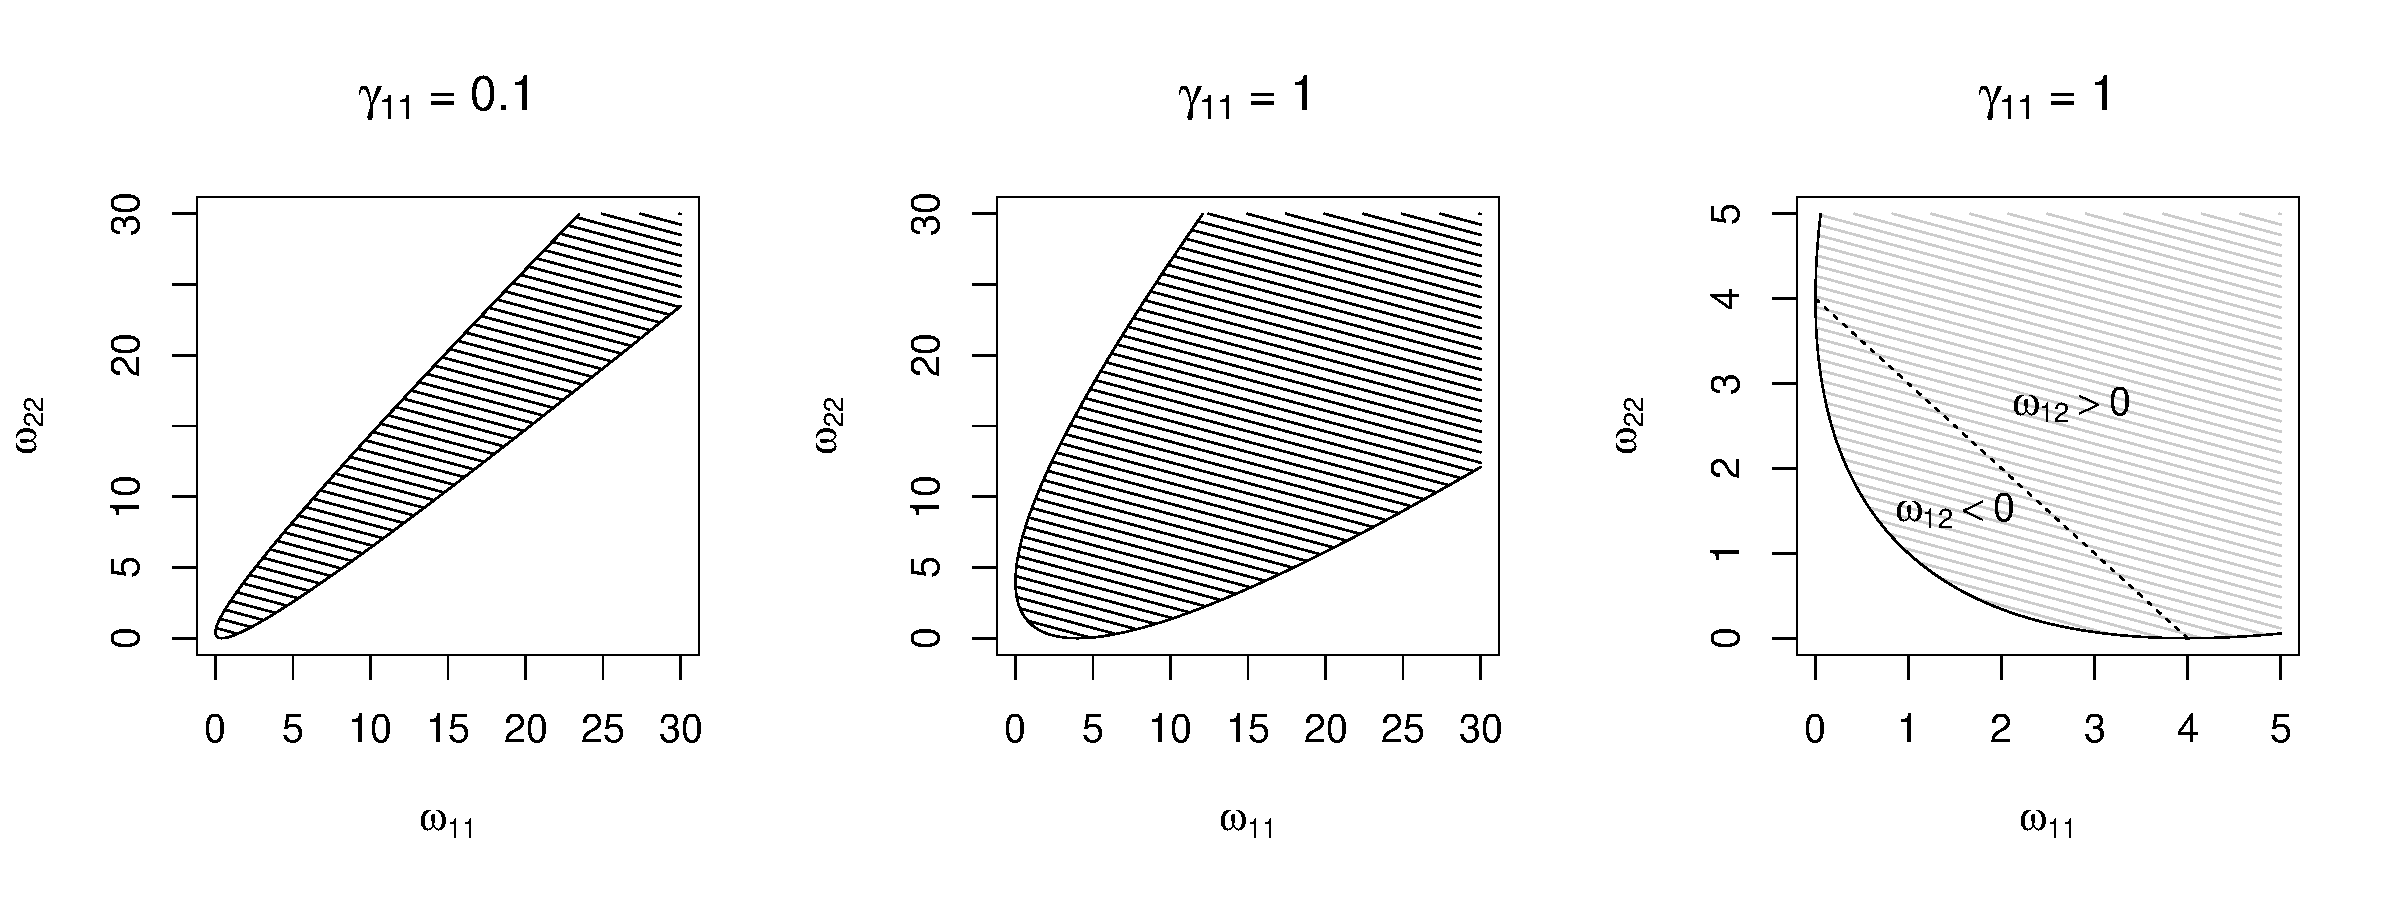
\includegraphics[width=6.5in]{figs/regions-2.pdf}
\begin{small}
\textit{Left and center: Region (shaded) where $\Omega$ is positive definite, for $\gamma_{11} = 0.1$ and $\gamma_{11} = 1$. Right: Subregions where $\log w_1$ and $\log w_2$ are negatively correlated, uncorrelated, and positively correlated. Along the dashed line, $\omega_{12} = 0$.}
\end{small}
\end{center}
\end{figure}

Near or at the boundary of the region, the correlation is near or equal to $\pm 1$. Along the line $\omega_{22} = \omega_{11}$, the correlation goes from $-1$ at $(\gamma_{11}, \gamma_{11})$ to 0 at $(2\gamma_{11}, 2\gamma_{11})$ and approaches $+1$ as $\omega_{11} = \omega_{22}$ increases.

\subsubsection*{Generalizing to Larger $p$}

Characterizing the region where $\Omega$ is positive definite is more difficult with $p > 2$, but the region can be explored for a particular $\Gamma$ by trial-and-error, choosing values for $\omega_{11}, \dots, \omega_{pp}$ and checking whether the minimum eigenvalue of $\Omega$ is positive (indicating positive definiteness).

Based on my investigation of several typical cases with moderately large $p$, it appears that $\Omega$ is positive definite for $(\omega_{11}, \dots, \omega_{pp}) = (\gamma_{11} + \delta, \dots, \gamma_{pp} + \delta)$ with any $\delta > 0$. For very small $\delta$, the off-diagonal entries of $\Omega$ are all or nearly all negative. As $\delta$ increases, the entries become all or nearly all positive. This pattern is similar to the pattern found in the $p = 2$ case.

It also appears to be true for larger $p$ that for fixed values of all $\omega_{ii}$ except one, say $\omega_{jj}$, $\Omega$ is positive definite only for a fairly small interval of $\omega_{jj}$ values.

The structure of $\Omega^{-1}$ appears to be stable over much of the region of positive definite $\Omega$ matrices. The partial correlations implied by $\Omega^{-1}$ vary little across $\Omega$ matrices sufficiently far from the boundary of that region. However, near the boundary of the region, where $\Omega$ becomes nearly singular, the partial correlations can change dramatically. Exactly how the partial correlations change, and how it relates to the hypothetical variances $\omega_{11}, \dots, \omega_{pp}$, needs more investigation.

What can be learned from these investigations is that for any given $\Gamma$ (or $\hat{\Gamma}$), there are potential log-absolute abundance covariance matrices which exhibit a wide variety of conditional and unconditional relationships, all resulting in the same $\Gamma$. What one would hope is that any valid $\Omega$ which is substantially different from $\Gamma$ represents an implausible covariance structure, and that any $\Omega$ which is plausible is also very similar to $\Gamma$, so that when graph selection is applied to the estimate of $\Gamma$, the inferences are similar to what one would obtain if the absolute abundances were available. However, one may have little idea about which covariance structures are plausible or not. The results here demonstrate a fundamental limitation of compositional data for inferring relationships among absolute abundances.

\subsection*{Graph Selection Performance}

\begin{figure}
\caption{Band, cluster, and scale-free graph structures used in $p = 64$ simulations.}
\label{f:graphs}
\begin{center}
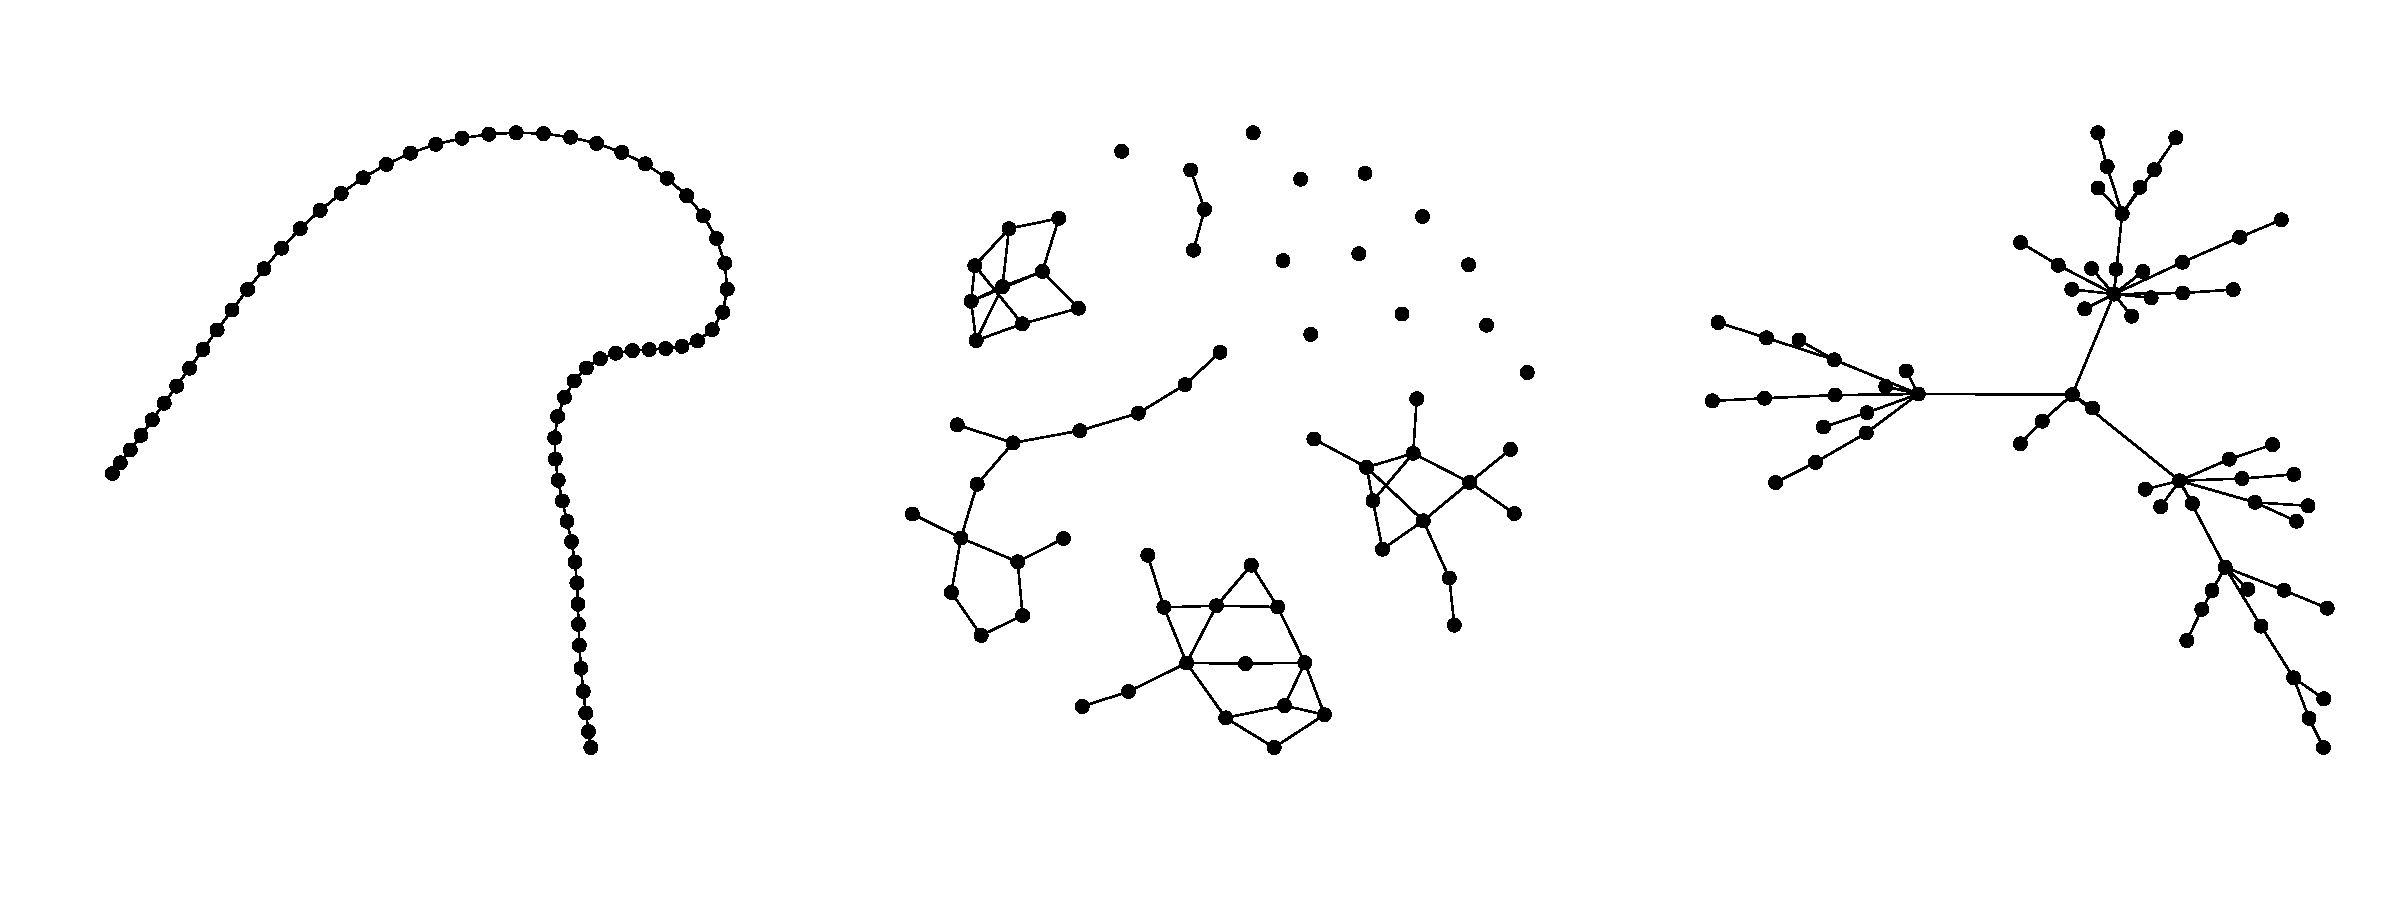
\includegraphics[width=6.5in]{figs/graphs-64.pdf}
\end{center}
\end{figure}

The following simulations show that graph selection based on compositional data can perform well if the compositionality does not have too strong an influence on covariances. Further simulations show that when the compositional effect is substantial, graph selection can perform very poorly.

To assess the performance of graph selection under ideal conditions, I ran simulations using log-normal absolute abundances so that the log-absolute abundances had a multivariate normal distribution. For $p = 64$ and $p = 256$, samples of size $n = 32$, $64$, $128$, $256$, or $512$ were generated using a fixed $\Omega^{-1}$ with the locations of non-zero entries determined by one of three graph structures (band, cluster, or scale-free) each with $p-1$ edges. The graphs for $p = 64$ are shown in Figure \ref{f:graphs}. To control the strengths of the conditional relationships, all diagonal entries in $\Omega^{-1}$ were 4 and all non-zero off-diagonal entries were $\pm 1$. Thus, the partial correlations were all equal to $\pm 0.25$. The signs of the $\Omega^{-1}$ entries were either all negative, half negative, or all positive. As noted above, a negative entry in the $(i,j)$ position of $\Omega^{-1}$ corresponds to a positive conditional dependence relationship between variables $i$ and $j$. That is, for fixed values of all other variables, variables $i$ and $j$ will have positive correlation when the entry in $\Omega^{-1}$ is negative and negative correlation when the entry is positive.

Performance was measured by the area under the precision-recall curve (AUPR) along the sequence of graphical lasso solutions for a decreasing sequence of $\lambda$ parameter values. Precision and recall are calculated based on the numbers of true positives (TP), false positives (FP), and false negatives (FN) as expressed below.
\begin{equation}
\text{Recall} = \frac{\text{TP}}{\text{TP}+\text{FN}}\ \ \ \text{Precision} = \frac{\text{TP}}{\text{TP}+\text{FP}}
\end{equation}
Here, a true positive is when an edge exists in the true graph and is selected by graphical lasso. A false positive is when the edge does not exist but is selected, and a false negative is when the edge does exist but is not selected. For comparison, AUPR was also measured for the graphical lasso solutions based on the log-abundance data before transformation.

This setup for the simulations was based on the simulations reported by Kurtz et al. \citeyear{kurtz}. The differences are that their simulations used count data mimicking microbial OTU counts from a real data set; they controlled the strength of OTU relationships using the condition number of the covariance matrix; for every $\Omega^{-1}$ entry in all trials, the sign was made positive with probability $\frac{1}{2}$ and negative otherwise; and they did not measure AUPR from the log-abundance data for comparison.

\begin{figure}
\caption{Graph selection performance with $p = 64$ and a scale-free graph structure.}
\label{f:perf64}
\begin{center}
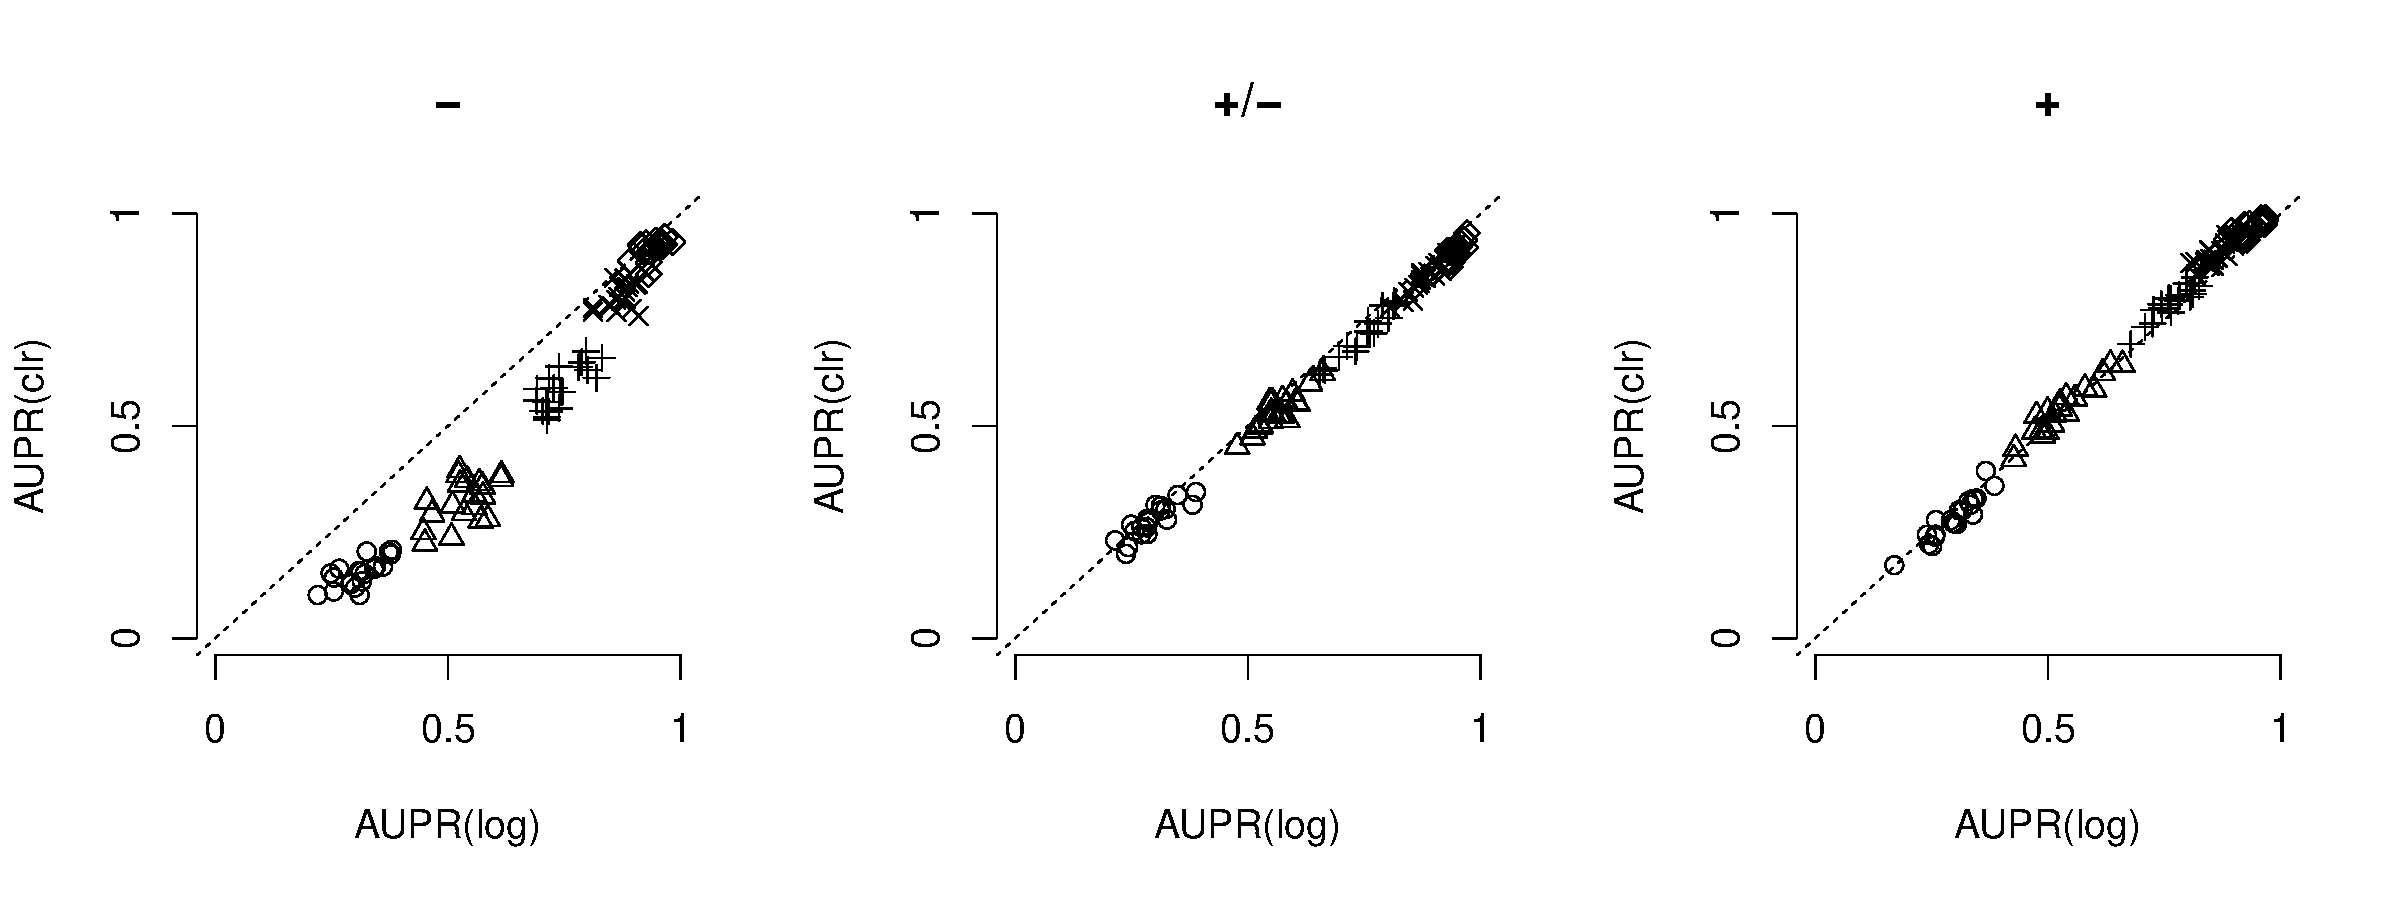
\includegraphics[width=6.5in]{figs/sim-64-scalefree.pdf}
\begin{small}
\textit{Different plotting characters correspond to different samples sizes. $-$, $+/-$, and $+$ refer to the signs of $\Omega^{-1}$ entries.}
\end{small}
\end{center}
\end{figure}

Besides sample size (performance steadily improved for both the log and clr data as $n$ increased from $32$ to $512$), the signs of $\Omega^{-1}$ entries had the largest effect on the performance of graph selection. For $p = 64$, when all of the $\Omega^{-1}$ entries were negative, graph selection using the clr-transformed abundances underperformed compared to graph selection using the log abundances (except for large $n$). The AUPR comparison for the scale-free graph is shown in Figure \ref{f:perf64}, and the comparison is similar for the other graph structures. However, for $p = 256$, performance is at least as good with clr data as with log data. Surprisingly, performance is sometimes slightly better with clr data for large $n$.

When all of the off-diagonal entries of $\Omega^{-1}$ are negative, all of the conditional relationships are positive, and the covariance matrix tends to have more and larger positive entries. This results in a larger difference between $\Gamma$ and $\Omega$, which seems to result in worse graph selection performance, though the effect diminishes with larger $p$.

\begin{figure}
\caption{Graph selection performance with one variance-dominating abundance.}
\label{f:prcurves}
\begin{center}
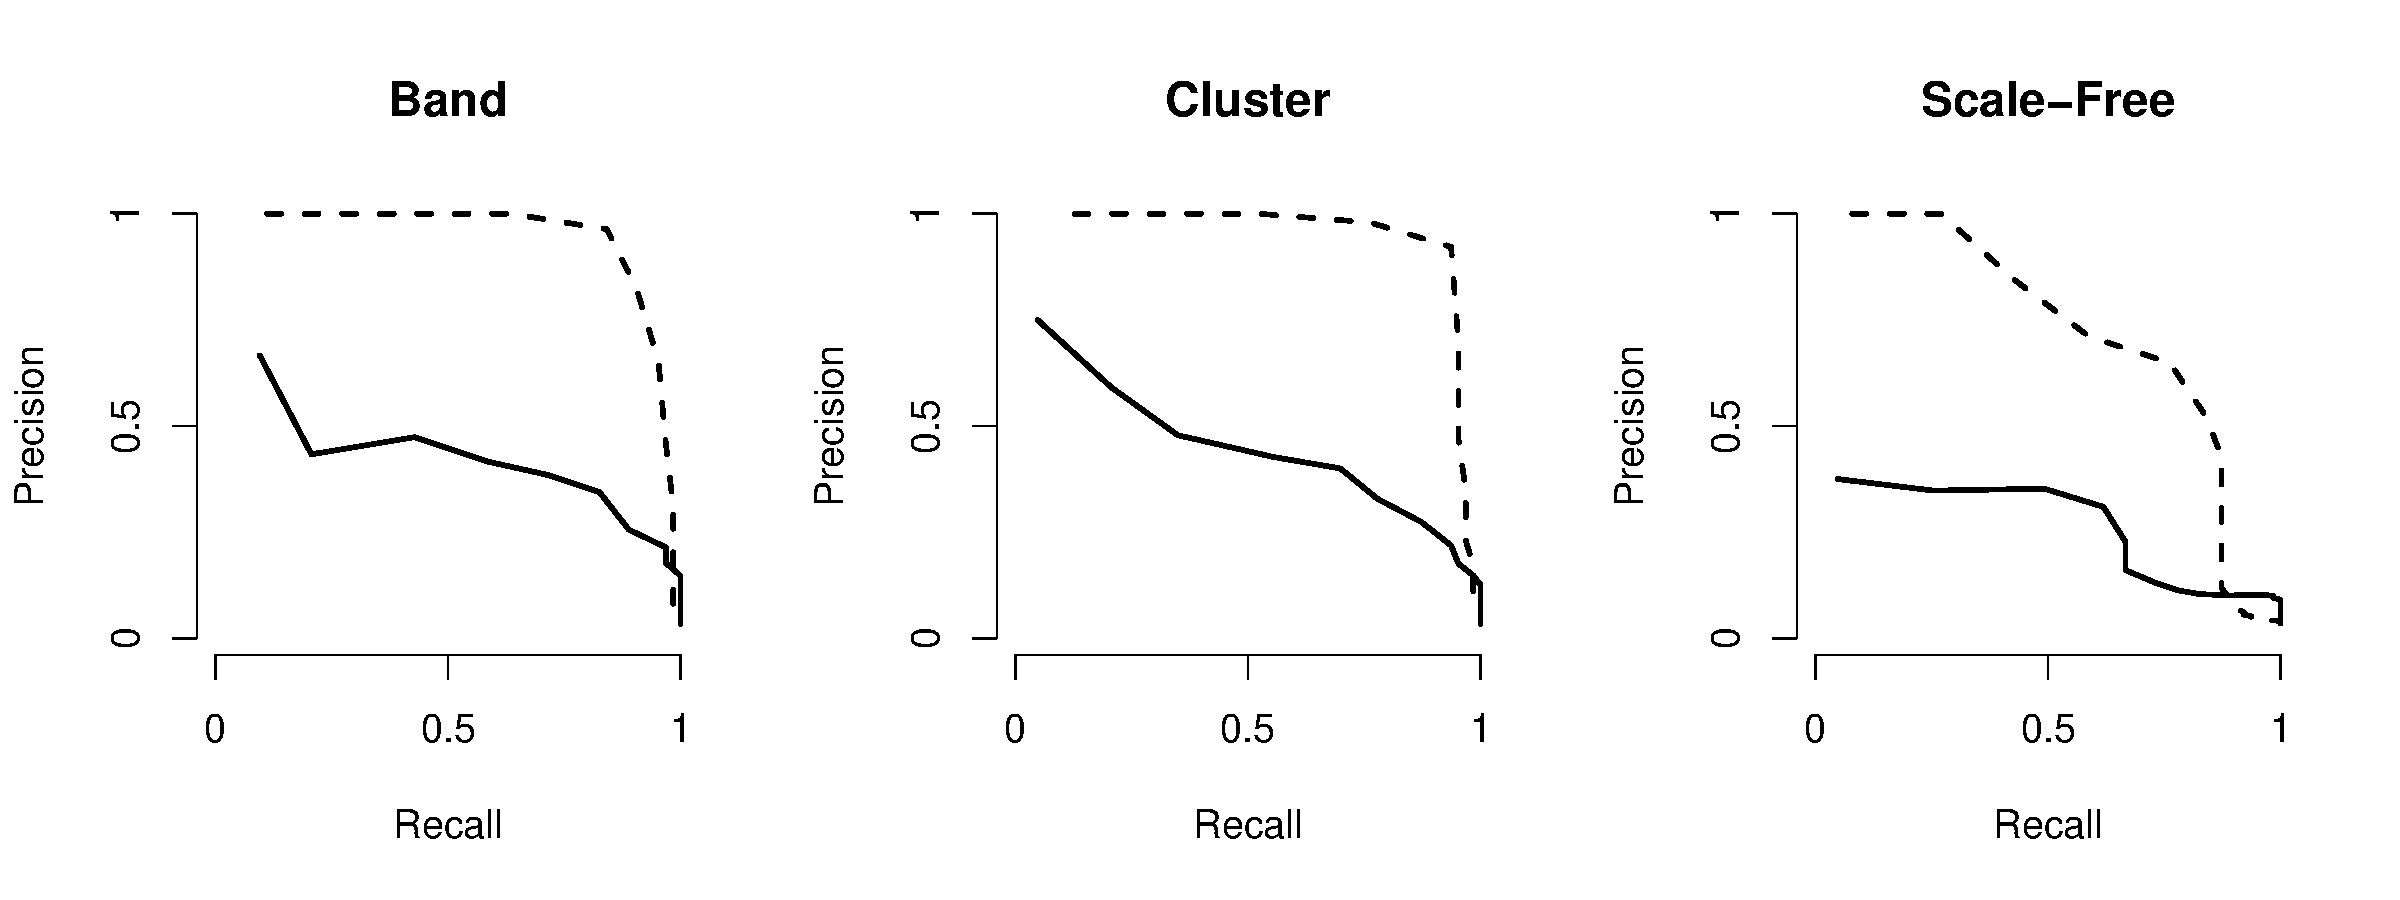
\includegraphics[width=6.5in]{figs/var-dom-pr.pdf}
\begin{small}
\textit{Precision vs. recall for graph selection from the clr} (-----) \textit{and log} (- - -) \textit{abundance data}.
\end{small}
\end{center}
\end{figure}

To test graph selection performance when the compositional effect is stronger, I used same $\Omega^{-1}$ from the $p = 64$ simulations above, but with the variance for $\log w_1$ set 400 times as large as the other variances.

Under these conditions, where the variance of $\sum_{i=1}^p \log w_i$ is dominated by $\log w_1$, graph selection performs much worse on the clr data than on the log data. Graphical lasso selects many spurious edges between $\log w_1$ and the other $\log w_i$ because the clr transformation induces substantial changes in the corresponding covariances. Precision-recall curves for each graph structure with $n = 256$ are shown in Figure \ref{f:prcurves}. The edges selected in the case of the band graph using the log data are compared to the edges selected using the clr data in Figure \ref{f:spurious}.

\begin{figure}
\caption{Spurious edges selected by graphical lasso.}
\label{f:spurious}
\begin{center}
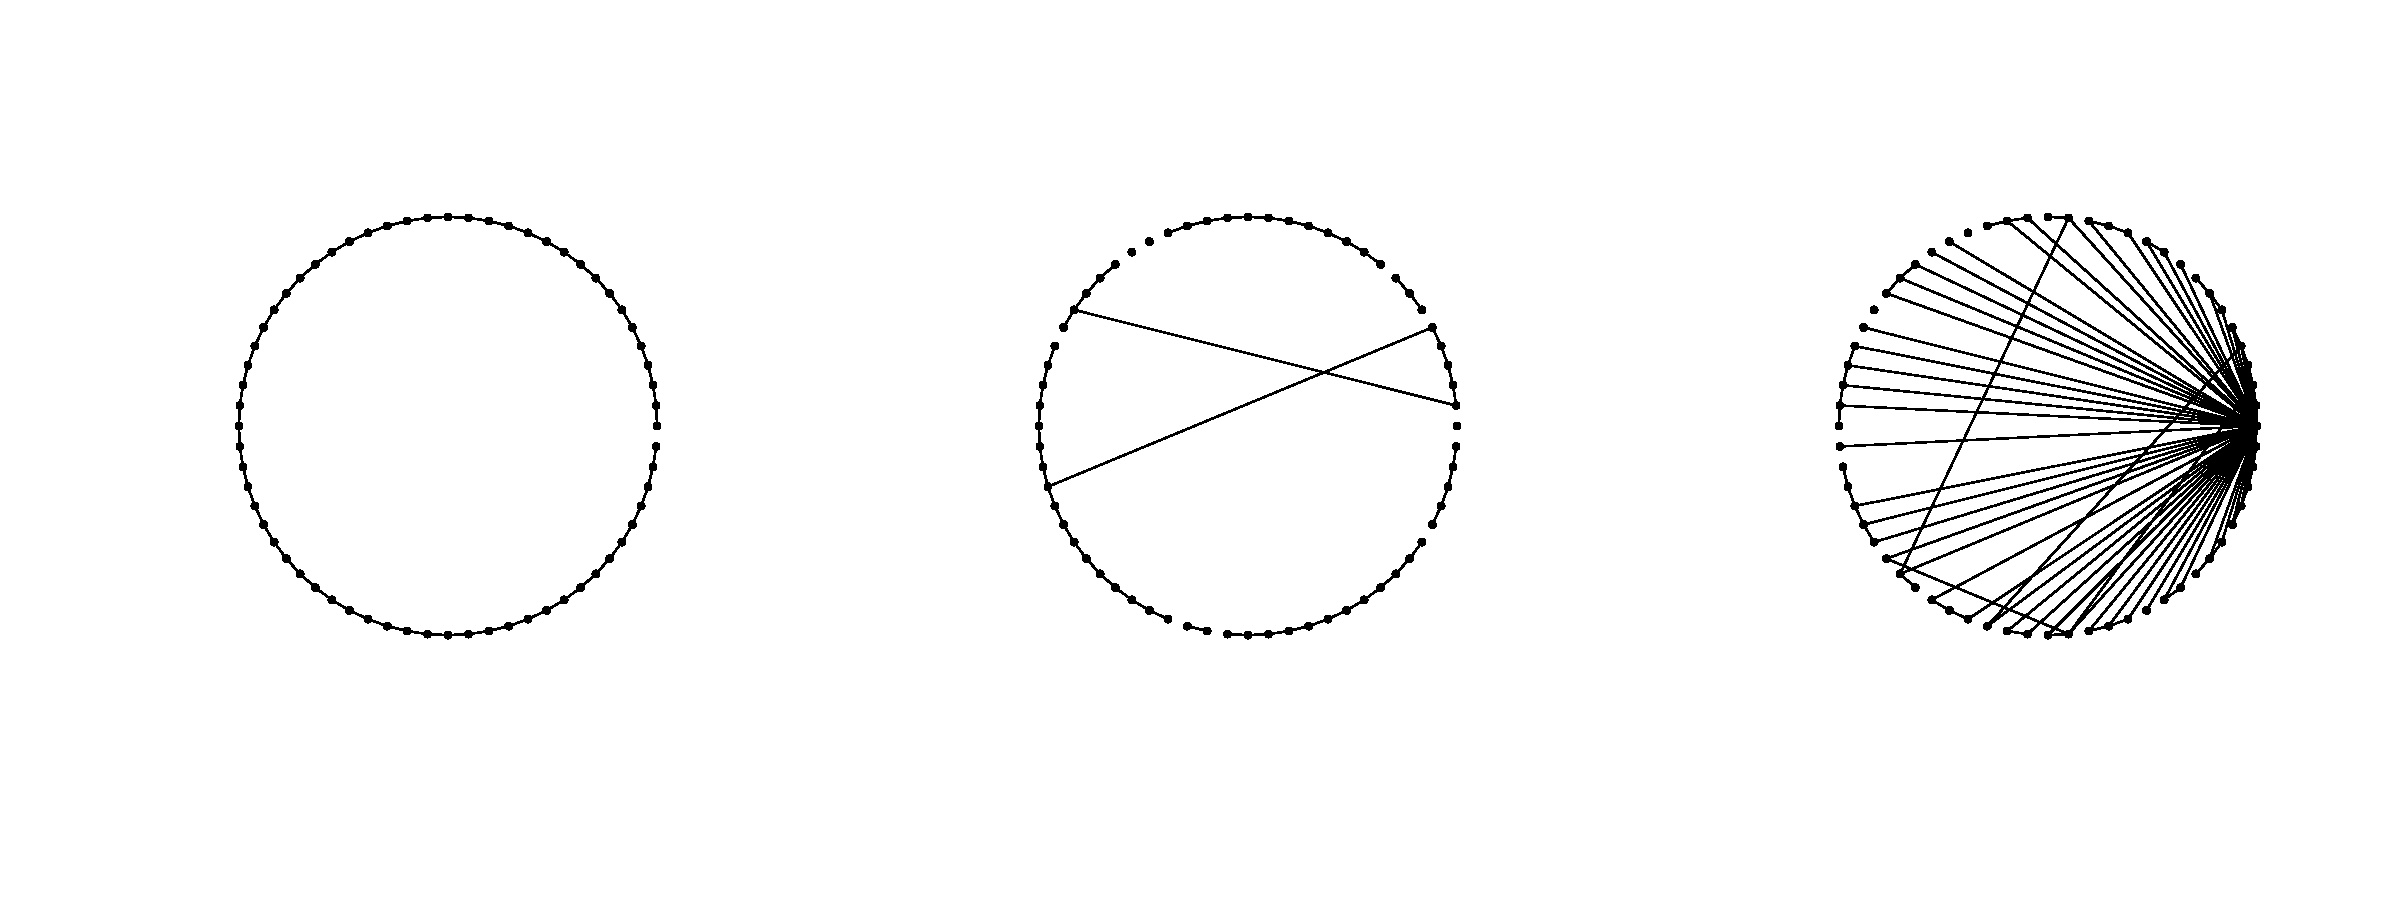
\includegraphics[width=6.5in]{figs/var-dom-band.pdf}
\begin{small}
\textit{Left: The true graph structure. Center: Edges selected by graphical lasso from the log abundance data, with lasso parameter $\lambda = 0.212$. Right: Edges selected from the clr abundance data with the same lasso parameter.}
\end{small}
\end{center}
\end{figure}

\subsection*{Conclusion}

Compositional data derived from absolute abundances are fundamentally limited in the information they provide about the absolute abundances. Any analysis which is based on covariances in the compositional data, as is the case with the graph selection method considered here, must be used with the recognition that covariances in the compositional data may differ substantially from covariances in the absolute abundances. I have found that a variety of absolute abundance covariance structures exhibiting very different types of relationships can result in the same covariance structure in the clr-transformed compositional data.

Based on simulations, graph selection using clr-transformed compositional data works as well as (and occasionally even better than) the graph selection that would result from the log abundances for large $p$, provided that the compositional effect is not too strong. Strong compositional effects result when, for example, one component or a group of components dominates the variance of the total abundance. Information about the total abundance is lost when absolute abundances become compositional, so whenever total abundance strongly depends on the abundance patterns of a subset of components, graph selection may perform poorly. If variances do not differ much and strong covariances are sparse, then moderate-to-large $p$ appears to be sufficient for the compositional effects to be diminished or negligible.

\pagebreak
\bibliographystyle{biom}
\bibliography{refs}

\end{document}
